\documentclass[11pt,a4paper]{article}
% rozmery stranky
\usepackage[left=1.5cm,text={18cm, 25cm},top=2.5cm]{geometry}
% cestina a fonty
\usepackage[czech]{babel}
\usepackage[utf8]{inputenc}
\usepackage[T1]{fontenc}
% dalsi balicky
\usepackage{graphicx}
\usepackage{enumitem}
\usepackage{indentfirst}
\usepackage{url}
\usepackage[bookmarksopen,colorlinks,plainpages=false,urlcolor=blue,
unicode,linkcolor=black]{hyperref}


\begin{document}

  \begin{titlepage}
    \begin{center}
      \Huge
      \textsc{Fakulta informačních technologií\\ Vysoké učení technické v~Brně}
      \vspace{100px}
      \begin{figure}[!h]
        \centering
        
\includegraphics[height=5cm]{logo}
      \end{figure}
      \\[50mm]
      \LARGE{Studie účelnosti zbudování vodní cesty Dunaj-Odra-Labe \,--\, 
             zadání č. 2}
      \vfill
    \end{center}
    \Large{Roman Blanco (xblanc01) \hfill 7.12.2014 \\
           Adam Jež (xjezad00)}
  \end{titlepage}

  \tableofcontents
  \newpage

  \section{Úvod}

    Cílem zadaného projektu bylo prostudovat zdroje, zabývající se účelností
    vybudování vodního koridoru Dunaj-Odra-Labe, a podle zjištěných údajů stanovit kvalifikovaný odhad roční poptávky po lodní přepravě mezi zvolenými uzly. Součástí zadání bylo také
    navrhnout a implementovat model dopravní cesty, včetně stavebních prvků.

    \subsection{Autoři}

      Autory projektu jsou Roman Blanco (xblanc01) a Adam Jež (xjezad00) \,--\,
      studenti 3. ročníku bakalářského studia na Fakultě Informačních
      technologii VUT v Brně. Prioritním zdrojem informací týkajících se zadaného tématu byly veřejně přístupné zdroje. Některé informace nám byly poskytnuty autory projektu zabývajícího se výstavbou koridoru.

    \subsection{Ověřování validity modelu}

      Ověřování validity modelu probíhalo pomocí experimentů, a to simulací ve virtuálním prostředí. Ověřovalo se,
      zda modelová situace odpovídá reálné situaci, přičemž informace
      byly čerpány pouze z věrohodných zdrojů. Jelikož reálný systém, určený simulovaným modelem v
      současné době neexistuje, jako validní jsme model prohlásili na základě získaných
      informací

  \section{Rozbor tématu}

    Informace, potřebné pro úspěšnou implementaci byly vyhledány na veřejně přístupných stránkách
    na internetu. Problémem při využívání těchto zdrojů byla skutečnost, že mnoho informací,
    bylo uvedeno pouze v sumarizovaných hodnotách za období celého roku. Pro některé hodnoty tak musel být použit kvalifikovaný odhad, podpořený údaji čerpanými ze statistik a dalších databází. Mimo již zmíněných veřejně přístupných webových stránek nám také často jako zdroj údajů posloužily diplomové či bakalářské práce. Níže je uveden souhrn hodnot, které jsme tímto způsobem získali:

    \noindent
    Hodnoty týkající se plavební komory:

    \begin{itemize}
      \item Doba uzavření vrat plavební komory je 60 sekund
      \item Doba otevření vrat plavební komory je 30 sekund
      \item Doba vplutí do plavební komory je 516 sekund
      \item Doba vyplutí z plavební komory je 355 sekund
      \item "Malá" plavební komora je taková, u níž výškový rozdíl mezi hladinami toku před a za komorou není větší než 12.5 m. Pokud plavební komora vyrovnává výšku hladiny přesahující 12.5 m, nazýváme ji "velkou" plavební komorou
      \item Napuštění nebo vypuštění 1 výškového metru "malé" plavební komory odpovídá doba 40 s
      \item Napuštění nebo vypuštění 1 výškového metru  "velké" plavební komory odpovídá doba 30,4 s
    \end{itemize}

    \noindent
    Hodnoty,týkající se plavby v tunelu:

    \begin{itemize}
      \item Odhadovaná rychlost lodi při plavbě v tunelu je 2,22 m/s

      \item Hranice, kdy se začne aplikovat seskupování je 3470 m
    \end{itemize}

    \noindent
    Hodnoty týkající se plavby v akvaduktu:

    \begin{itemize}
      \item Rychlost při plavbě v tunelu je 2,77 m/s
      \item Hranice, kdy se začne aplikovat seskupování je 2090 m
    \end{itemize}

    \noindent
    Obecné hodnoty při plavbě:

    \begin{itemize}
      \item Rychlost plavby v kanálu je 3,33 m/s
      \item Rychlost plavby po proudu toku řeky je 4,16 m/s
      \item Rychlost plavby proti proudu toku řeky je 1,66 m/s
      \item Maximální náklad lodi je 4000 tun
    \end{itemize}
        
    Jako prioritní zdroj informacím o plánované trase koridoru 
    nám velmi dobře posloužily volně
    dostupné materiály na internetové stránce projektu zabývajicího se
    problematikou koridoru Dunaj-Odra-Labe a také poskytnuta literatura od
    týchž autorů [1].

    \begin{figure}[ht!]
      \centering
      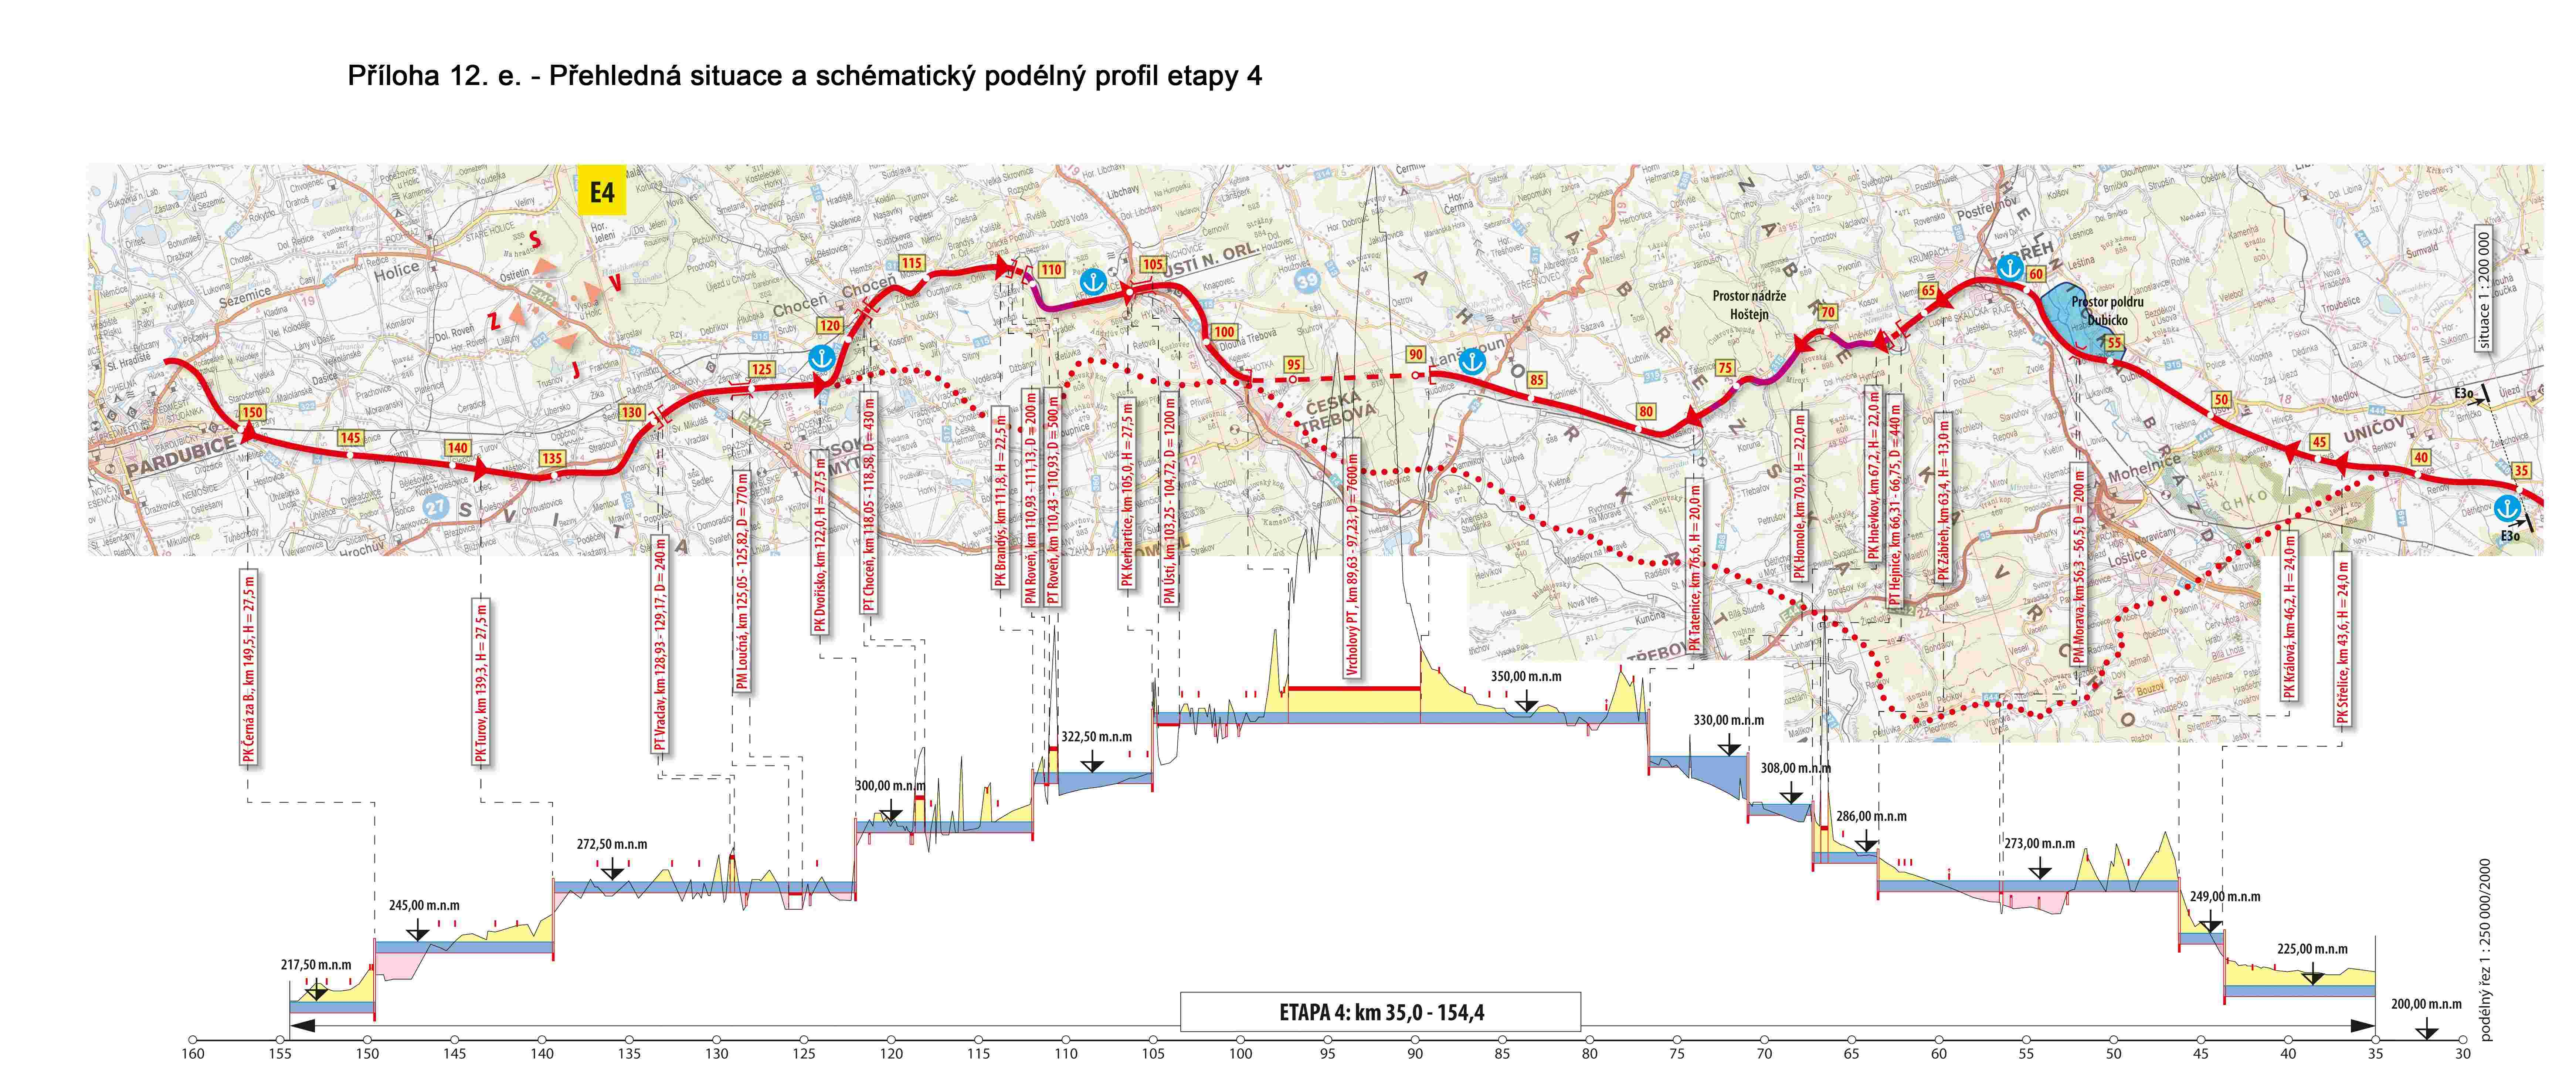
\includegraphics[width=1\textwidth, natwidth=6969, natheight=2953]
                      {etapa4.jpg}
      \caption{A simple caption \label{overflow}}
    \end{figure}

  \section{TODO: jak je to vymodelovane}

    Lodi v tunelu se nemohou pohybovat proti sobě
    Lodi, které se chystají projet tunelem stejným směrem, se mohou seskupit za účelem zrychlení plavby

  \section{Závěr}

  \section{Reference}

    \begin{enumerate}[label={[\arabic*]}]
      \item Mapy s etapami výstavby koridoru 
        \href{http://d-o-l.cz/index.php/cs/kestazeni/category/14}
             {d-o-l.cz}
      % experimentalni zdroj, ale udaje souhlasi s oficialnimi
      \item Plánovaná trasa koridoru zaznačená v Google Maps
        \href{http://povode.aspone.cz/Maps/dol.html}
             {povodne.aspone.cz/Maps/dol.html}
    \end{enumerate}

  \appendix
    \newpage

  \section{Přílohy}

\end{document}
